\chapter{Evaluation}
To measure the performance of our algorithm, we evaluated \todor{werden tests evaluiert, oder algorithmen?} it on custom synthetic \textit{labeled} data sets, generated via the method mentioned in \autoref{sec:datagen}, which serves as the \textit{groundtruth} of our data. Explicitly we compared our novel algorithm with its ancestor \gls{cash} in clustering and runtime performance in various settings we will mention later. Since clustering is an unsupervised setting and the different clustering algorithms do not label the clusters uniformly with the same schema/value, we chose to compare the clustering labels via the \gls{ari}\cite{hubert1985comparingari} and \gls{nmi}\cite{strehl2002clusternmi} score, which are invariant to the permutations of the labeling. Later in this chapter we review the available hyperparameters of our algorithm and, based on previously evaluated data, explain their impacts on the performance.

The algorithms and evaluation are implemented in \textit{python v3.7.4}. Each of the data sets locally dense correlations are uniquely labeled and previously pruned noise points relabeled to a nearby linear correlation if the point was within a certain vicinity from the correlation away. For the density-based clustering we applied \gls{optics} from \textit{scikit-learn v0.21.2}\cite{pedregosa2011scikit} and for the extraction of the correlations we utilized \gls{cash} from the data mining tool \textit{\gls{elki} v0.7.5}\cite{achtert2008elki}. 

% We defined the threshold of the vicinity as $jitter_{thres}$ which merges the noise points if the euclidean distance to a nearby linear correlation $distance_{point\rightarrow hyperplane} = \frac{\Vec{n}\cdot\Vec{x}+\delta}{|\Vec{n}|}$ is smaller than the threshold. These data sets are served as our \textit{groundtruth}. Based on these groundtruths we compared our local-global combining clustering approach's results with its ancestor \gls{cash}'s results in the accuracy of their labeling based on the \gls{ari} and \gls{nmi} score and its runtime performance.

\todor{reichen 2d veranschaulichungen? 3d is hard}

\section{Setup}\label{sec:setup}

Our test setups were conducted on $d$-dimensional synthetic data sets with four characteristic jittery $d-1$-dimensional correlations, i.e. partial, intersecting and/or parallel correlations. The tests consisted of the evaluation of the algorithms different behaviours w.r.t runtime, \gls{ari} and \gls{nmi} scoring for different amount of points/objects, different dimensionalities and seven different levels of noise (0, 1, 5, 10, 25, 40, 80).

All following tests were executed in docker containers running on a Virtual Machine with an x86\_64 bit architecture, 48 CPUs (2 GHz) and 246GB RAM. 

\begin{figure}
    \centering
    \begin{minipage}[t]{.5\textwidth}
    \centering
    \captionsetup{width=.9\linewidth}
    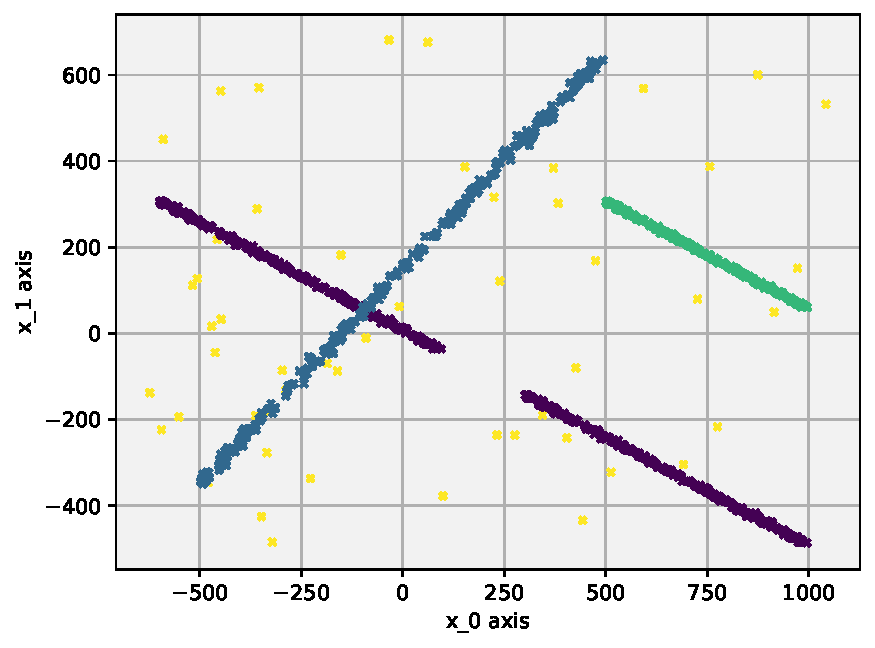
\includegraphics[width=\textwidth]{evalfigures/2DSetGrid.pdf}
    \captionof{figure}{Insight into clustering structure in 2D and 3D}
    \label{fig:my_label}
    \end{minipage}%
    \begin{minipage}[t]{.5\textwidth}
    \centering
    \captionsetup{width=.9\linewidth}
    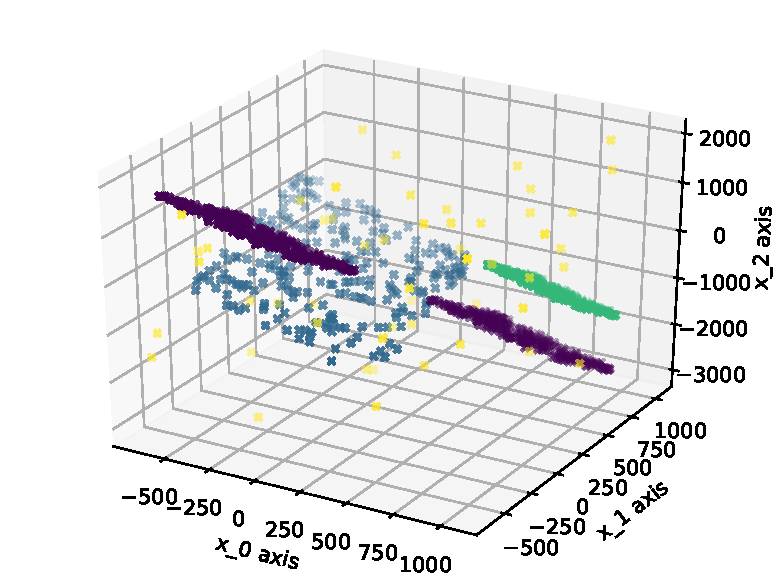
\includegraphics[width=\textwidth]{evalfigures/3DSet.pdf}
    \captionof{figure}{Insight into clustering structure in 2D and 3D}
    \label{fig:my_label}
    \end{minipage}%
\end{figure}

% The algorithms and evaluation are implemented in \textit{python v3.7.4}. Each of the data sets locally dense correlations are uniquely labeled and previously pruned noise points relabeled to a nearby linear correlation if the point was within a certain vicinity from the correlation away. For the density-based clustering we applied \gls{optics} from \textit{scikit-learn v0.21.2}\cite{pedregosa2011scikit} and for the extraction of the correlations we utilized \gls{cash} from the data mining tool \textit{\gls{elki} v0.7.5}\cite{achtert2008elki}. 

% (which data sets have been used? How many data objects? How many clusters? Which programming language and libraries? On which hardware?) [0.5]
\section{Performance}
 To evaluate the performance of our algorithm compared to \gls{cash} we performed up to 500 iterations of random parameter search on each data set while tracking runtime for a measure of efficiency and scoring the effectivity based on the \gls{ari} and \gls{nmi} score compared to our prelabeled groundtruth. However due to time constraints we bounded the maximal time for all iterations to a maximum of 24 hours. \todor{unsicher ob das rein soll}
 
\begin{table}[]
\centering
\resizebox{\textwidth}{!}{%
\begin{tabular}{@{}llll@{}}
\toprule
Test setting           & Dimensions & Noise in \% & \# of objects \\ \midrule
Increasing objects    & 3D         & 5           & -             \\
Increasing dimensions & -          & 5           & 10000         \\
Increasing noise      & 3D         & -           & 10000         \\ \bottomrule
\end{tabular}%
}
\caption{}
\label{tab:reducedsetup}
\end{table}
 
\subsection{Efficiency}
 The evaluation of runtime performance measures the average runtime of the three different settings for both local (our algorithm) and global (default \gls{cash}) approaches. 
 
% \begin{figure}[ht]
%     \centering
%     \begin{minipage}[t]{.5\textwidth}
%       \centering
%       \captionsetup{width=.9\linewidth}
%       \includegraphics[width=.9\textwidth]{evalfigures/Avg_Runtime_3D_N5_pobjects_bar.pdf}
%       \captionof{figure}{a) Runtime per number of objects}
%       \label{fig:eval_per_dim}
%     \end{minipage}%
%     \begin{minipage}[t]{.5\textwidth}
%       \centering
%       \captionsetup{width=.9\linewidth}
%       \includegraphics[width=.9\textwidth]{evalfigures/Average_Duration_per_Noise.pdf}
%       \captionof{figure}{b) Second}
%       \label{fig:eval_per_noise}
%     \end{minipage}    \begin{minipage}[t]{.5\textwidth}
%       \centering
%       \captionsetup{width=.9\linewidth}
%       \includegraphics[width=.9\textwidth]{evalfigures/Average_Duration_per_Dimension.pdf}
%       \captionof{figure}{a) First}
%       \label{fig:eval_per_dim}
%     \end{minipage}%
%     \begin{minipage}[t]{.5\textwidth}
%       \centering
%       \captionsetup{width=.9\linewidth}
%       \includegraphics[width=.9\textwidth]{evalfigures/Average_Duration_per_Noise.pdf}
%       \captionof{figure}{b) Second}
%       \label{fig:eval_per_noise}
%     \end{minipage}
% \end{figure}
\begin{figure}
    \centering
    \includegraphics[width=0.8\textwidth]{evaluation/Avg_Runtime_3D_N5_pobjects_bar.pdf}
    \caption{Caption}
    \label{fig:eval_per_objects}    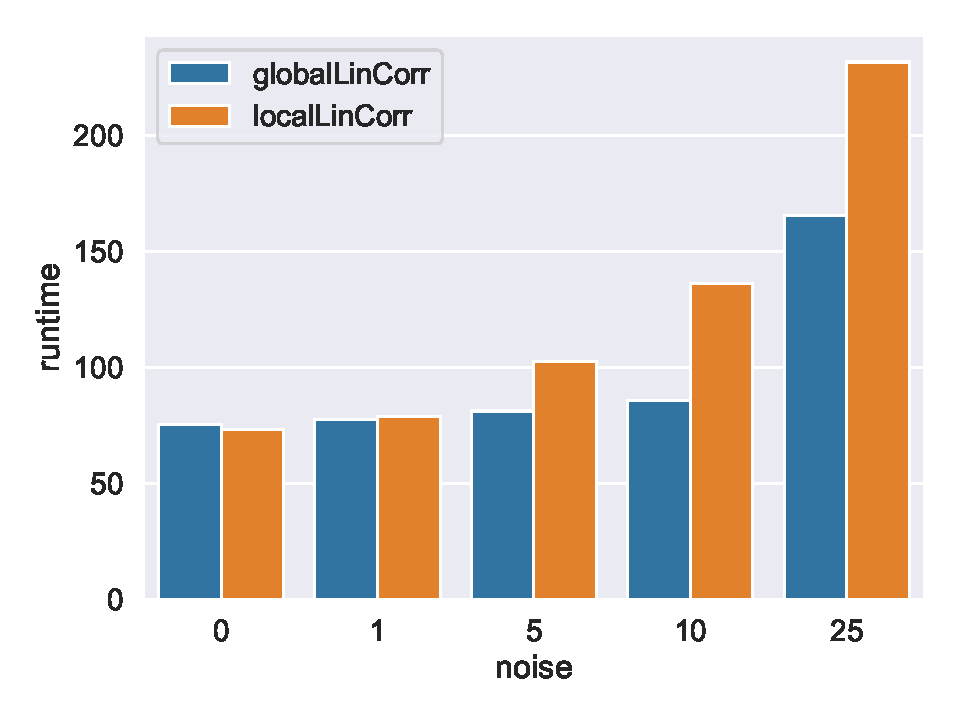
\includegraphics[width=0.8\textwidth]{evaluation/Avg_Runtime_3D_O10000_pnoise_bar.pdf}
    \caption{Caption}
    \label{fig:eval_per_noise}
\end{figure}

\autoref{fig:eval_per_objects} shows the average runtime of both algorithms w.r.t. the \textit{number of objects} in the 3-dimensional clusters of the data set with 5 percent noise respective to the data set size. Here our algorithm scales comparably to \gls{cash} even improves in runtime performance with a higher number of objects. 

% \begin{figure}[h]
%     \centering

% \end{figure}
The results of the average runtime w.r.t the different dimensionalities of the data space is depicted in \autoref{fig:eval_per_dim}.

\autoref{fig:eval_per_noise} shows the average runtime of our algorithm w.r.t. the noise percentage of the data sets.
 
\subsection{Effectiveness}
For clustering performance measures we took the best parameter sets of previous efficiency evaluation for both local and global approach and stacked their \gls{ari} and \gls{nmi} scores up against each other.

\begin{figure}[h]
    \centering
    \begin{minipage}[t]{.5\textwidth}
      \centering  
      \captionsetup{width=.9\linewidth}
      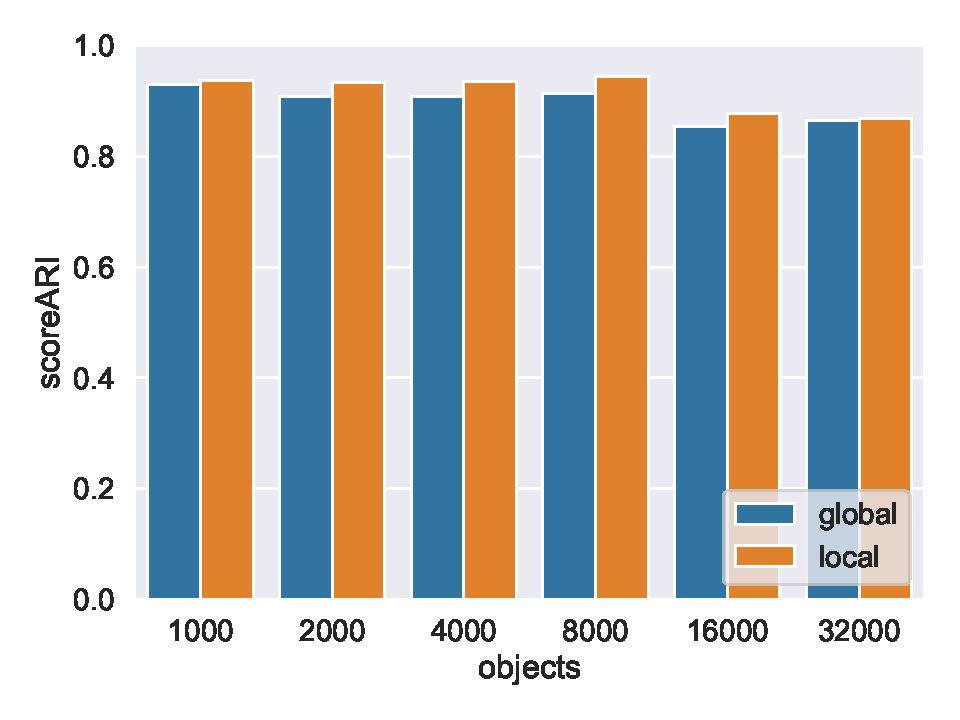
\includegraphics[width=\textwidth]{evaluation/Best_ARI_3D_N5_pobjects_bar.pdf}
      \captionof{figure}{a) First}
      \label{fig:ariperpts}
    \end{minipage}%
    \begin{minipage}[t]{.5\textwidth}
      \centering
      \captionsetup{width=.9\linewidth}
      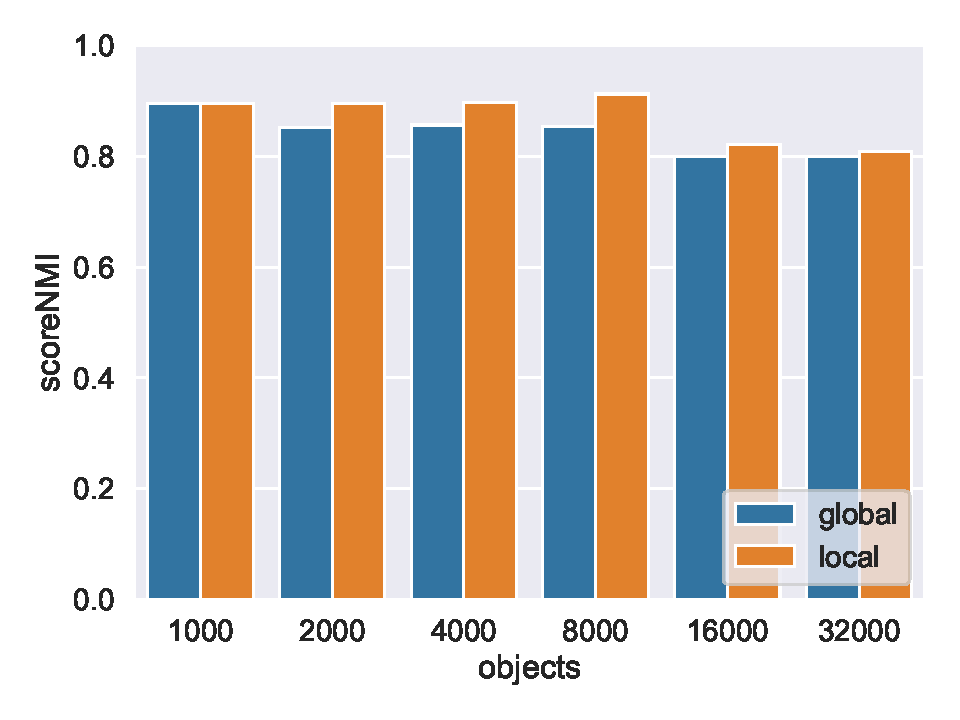
\includegraphics[width=\textwidth]{evaluation/Best_NMI_3D_N5_pobjects_bar.pdf}
      \captionof{figure}{b) Second}
      \label{fig:nmiperpts}
    \end{minipage}
\end{figure}
\begin{figure}[h]
    \centering
    \begin{minipage}[t]{.5\textwidth}
      \centering  
      \captionsetup{width=.9\linewidth}
      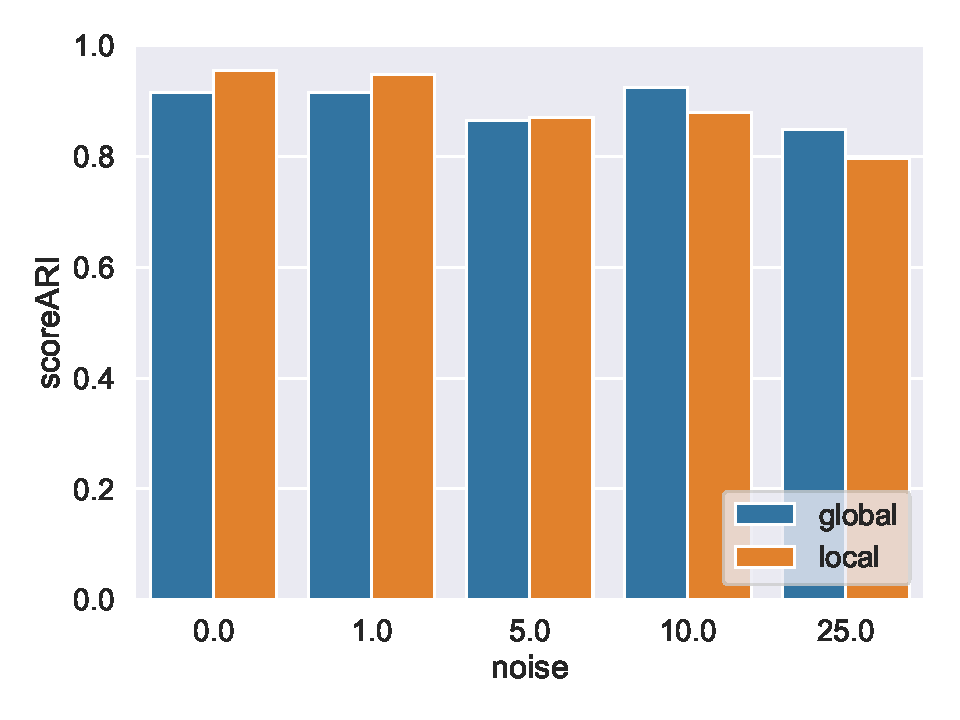
\includegraphics[width=\textwidth]{evaluation/Best_ARI_3D_O10000_pnoise_bar.pdf}
      \captionof{figure}{a) First}
      \label{fig:ariperpts}
    \end{minipage}%
    \begin{minipage}[t]{.5\textwidth}
      \centering
      \captionsetup{width=.9\linewidth}
      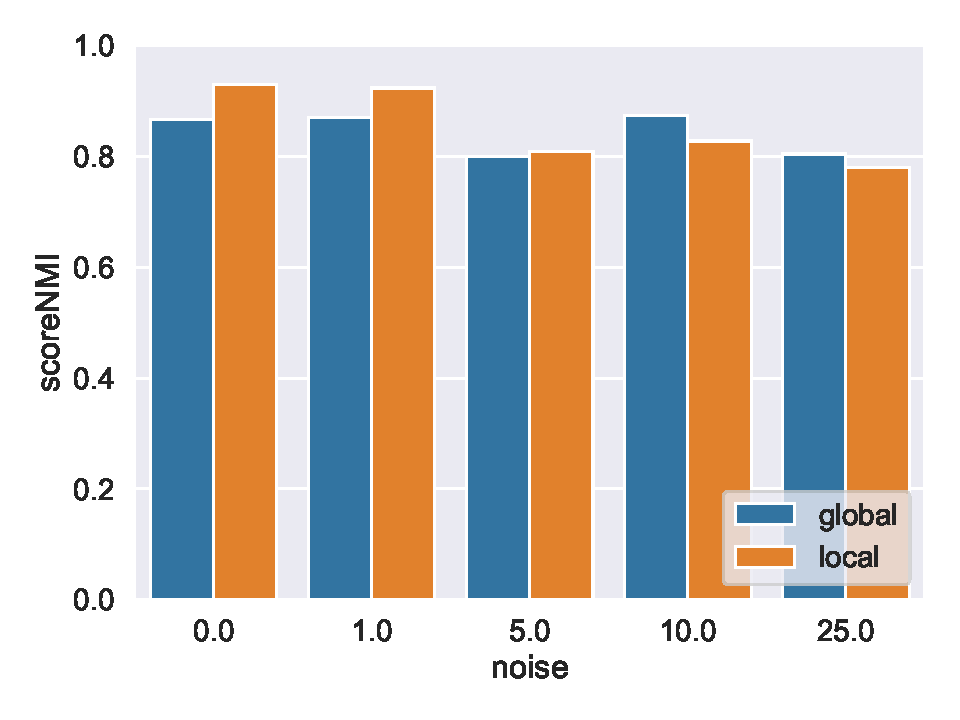
\includegraphics[width=\textwidth]{evaluation/Best_NMI_3D_O10000_pnoise_bar.pdf}
      \captionof{figure}{b) Second}
      \label{fig:nmiperpts}
    \end{minipage}
\end{figure}

\section{Parameters available and their impacts}
Our algorithm depends on many components such as \gls{optics} and \gls{cash} which come with several parameters themselves. In this section we discuss their meaning and their impact for the clustering results.

\subsection{Metrics: CosineSimiliarity(n1,n2), CosineSimiliarity(n1,n2) + EuclidianDistance(d) [2-3]}

\subsection{Median vs.  Mean}

\section{Results between Dense approach with stitching and Global approach}

\section{Test on real world data set(s) [1]}

%evtl. "Hyperparameter sensitivity" d.h. wie 'empfindlich' ist das verfahren bzgl. welchen Parameter Einstellungen?